\documentclass[11pt,a4paper]{article}
\usepackage[margin=2.4cm]{geometry}
\usepackage{amsmath,amssymb,graphicx,booktabs,hyperref}
\title{A070 v0.2.1: Strict Synthetic Blind Patch\\Absolute-Time Torsional-Light Falsifier}
\author{SST exploratory research pilot -- not certified}
\date{18 October 2026}
\begin{document}
\maketitle
\begin{abstract}
The prior v0.2.0 model selected the unmotivated angle $50^\circ$ and used $\Omega=|\mathbf{v}_{\!\boldsymbol{\circlearrowleft}}|/r_c$, making its SI group-speed result dependent on the canonical scale input. Version 0.2.1 freezes the angle sequence and nondimensional wave numbers before classifying five masked synthetic families. This is a blinded mechanism-discrimination control, not independent PKLSA validation or a photon discovery.
\end{abstract}
\section{Fundamental SST distinctions}
Absolute time $t$ parametrizes the incompressible Euler background. Local Swirl-Clock time $\tau_i$ and operational length $\ell_{\mathrm{op},i}$ are internal observables, not identical to absolute Euclidean distance $x$ or absolute time. With $f_i=d\tau_i/dt$ and direction-dependent $A_i=d\ell_{\mathrm{op},i}/dx$, the identity $c_{\rm local}=(A_i/f_i)c_{\rm abs}$ does not by itself determine any factor. No such factor enters the blind classifier.
\section{Reference equations and controls}
\begin{align}
\partial_t\mathbf u+(\mathbf u\cdot\nabla)\mathbf u&=-\frac{1}{\rho_{\!f}}\nabla p,\qquad \nabla\cdot\mathbf u=0,\\
\omega_\pm(\mathbf{k})&=\pm\frac{2\boldsymbol{\Omega}\cdot\mathbf k}{|\mathbf k|},\\
\mathbf v_g&=2\left[\frac{\boldsymbol{\Omega}}{|\mathbf k|}-\frac{(\boldsymbol{\Omega}\cdot\mathbf k)\mathbf k}{|\mathbf k|^3}\right],\qquad \mathbf k\cdot\mathbf v_g=0.
\end{align}
At $\theta=90^\circ$ the inertial frequency vanishes, so the group-velocity formula must not be interpreted as a validated photon transport mode there. Under uniform advection, $\omega_{\rm lab}=\omega_{\rm intrinsic}+\mathbf k\cdot\mathbf U$.
\section{Frozen design}
Seven angles $\{0,15,30,45,60,75,90\}^\circ$ and five nondimensional wave numbers $\{0.25,0.5,1,2,4\}$ are checked. The blind engine fits absolute temporal frequencies to the preregistered shape families: stationary $0$, passive axial advection $a k|\cos\theta|$, rotating inertial reference $a|\cos\theta|$, imposed isotropic linear positive control $ak$, and unknown. The imposed linear control has no Euler-based status.
\begin{center}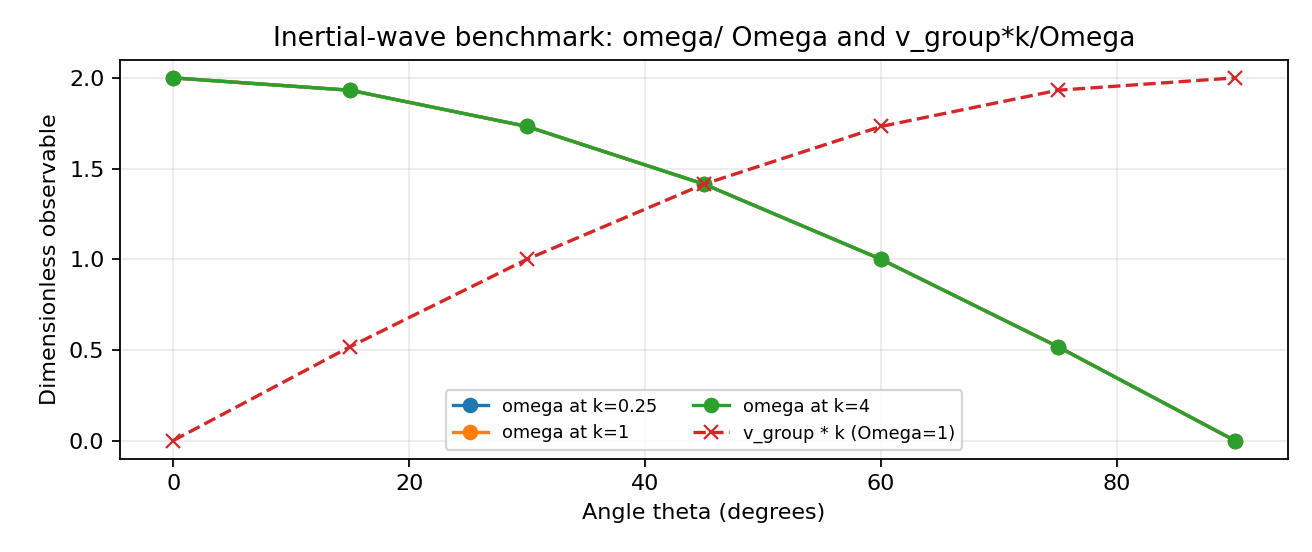
\includegraphics[width=.86\linewidth]{figures/predeclared_angle_scan.png}\end{center}
\section{Blinding and gating}
Masked time series, frozen predictions and a SHA-256 input manifest are shipped separately from reveal truth. The frozen classification digest can be verified without unblinding. The classification run passed, and 13 regression tests passed. These are synthetic results, not real observational independence. Native finite-core PKLSA modes, $f_i$, $A_i$, relativistic moving-observer light closure, gravity and cosmological tests remain unresolved. The software is not a certified frozen-framework v1.0.7 instance.
\begin{center}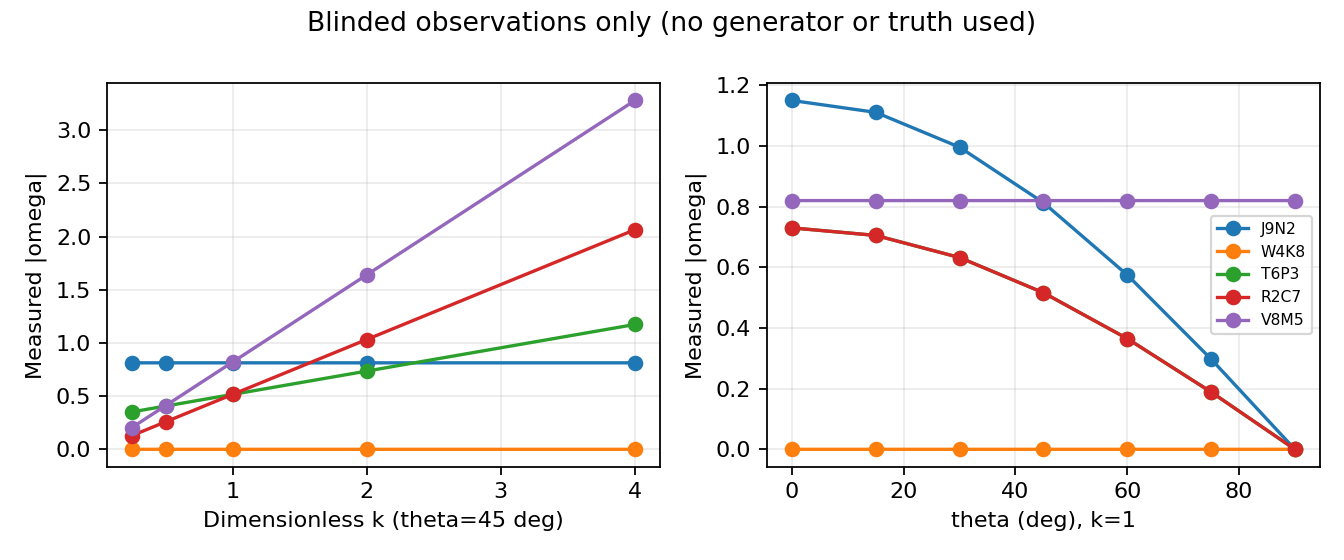
\includegraphics[width=.86\linewidth]{figures/masked_reference_scans.png}\end{center}
\section{Bibliography}
\begin{thebibliography}{99}
\bibitem{Batchelor1967} G. K. Batchelor (1967), \emph{An Introduction to Fluid Dynamics}, Cambridge University Press, DOI: \href{https://doi.org/10.1017/CBO9780511800955}{10.1017/CBO9780511800955}.
\bibitem{Greenspan1968} H. P. Greenspan (1968), \emph{The Theory of Rotating Fluids}, Cambridge University Press, ISBN 9780521043885.
\bibitem{Saffman1992} P. G. Saffman (1992), \emph{Vortex Dynamics}, Cambridge University Press, DOI: \href{https://doi.org/10.1017/CBO9780511624063}{10.1017/CBO9780511624063}.
\bibitem{Ashby2003} N. Ashby (2003), ``Relativity in the Global Positioning System,'' \emph{Living Reviews in Relativity} 6, 1, DOI: \href{https://doi.org/10.12942/lrr-2003-1}{10.12942/lrr-2003-1}.
\end{thebibliography}
\end{document}
